\documentclass[12pt]{article}
% \usepackage[brazilian]{babel}
\usepackage[a4paper,inner=1.5cm,outer=1.5cm, total={6in, 8in}]{geometry}
\usepackage[utf8]{inputenc}
\usepackage{lmodern}
\usepackage{graphicx}
\usepackage{float}
\usepackage{newtxmath}
\usepackage{amssymb, amsmath, amsfonts, array}
\usepackage{bm}
\usepackage{indentfirst}

\title{TIP8419 - Tensor Algebra\\ 
       Homework 2}
\author{Ezequias Márcio - $497779$}
\date{\today}

\begin{document}

\maketitle

\section*{Khatri-Rao Product}\vspace{.5cm}

\noindent
\textbf{Problem 1.} Generate $\bm{X} = \bm{A}\diamond\bm{B} \in 
\mathbb{R}^{I^2 \times R}$, for randomly chosen  
$\bm{A} \in \mathbb{R}^{I\times R}$ and $\bm{B}\in \mathbb{R}^{I\times R}$. 
Compute the left pseudo-inverse of $\bm{X}$ and obtain a graph that shows the 
run time vs. number of rows $(I) $ for the following methods:

\begin{itemize}
    \item [(a)] Method 1: Matlab/Octave/Python(Numpy) $\text{pinv}(\bm{X})= 
    \text{pinv}(\bm{A}\diamond \bm{B})$

    \item [(b)] Method 2: $(\bm{X}^{\dagger} = \big( \bm{X}^T\bm{X}\big) 
    \bm{X}^T = \big[\big(  \bm{A}\diamond \bm{B} \big)^T
    \big(  \bm{A}\diamond \bm{B} \big)
    \big]^{-1}\big( \bm{A}\diamond \bm{B} \big)^T$\\
    
    \item [(c)] Method 3: $(\bm{X}^{\dagger} =
    \big[\big(  \bm{A}\diamond \bm{B} \big)^T
    \big(  \bm{A}\diamond \bm{B} \big)
    \big]^{-1}\big( \bm{A}\diamond \bm{B} \big)^T = 
    \big[\big( \bm{A}^T \bm{A} \big) \odot
    \big(  \bm{B}^T \bm{B} \big)\big]^{-1}
    \big( \bm{A}\diamond \bm{B} \big)^T$
\end{itemize}

\noindent \textbf{Solution:}\\

%------------------------------------------------------------------------------
The algorithm used to calculate these Khatri-Rao product pseudo inverses in 
this work was implemented in \texttt{python} and it can be found in the files 
\texttt{tensoralg.py} and \texttt{hw1\_presentation.ipynb}. 
The run time curves are result of a Monte Carlo simulation with 
$100$ realizations that was implemented in the file 
\texttt{hw2\_presentation.ipynb} for each problem.

In Figure \ref{r2}, we can see the difference of execution time between 
the two strategies to calculate the pseudo-inverses varying the number of rows 
$I \in \{2,4,8,16,32,64,128,256\}$ for the case where the matrices have $R = 2$ 
columns.

For the case with $R=2$ the method $3$ presented a better performance as 
expected for deal with less complex operations exploiting the properties of the 
Khatri-Rao product. 

\begin{figure}[H]
    \centering 
    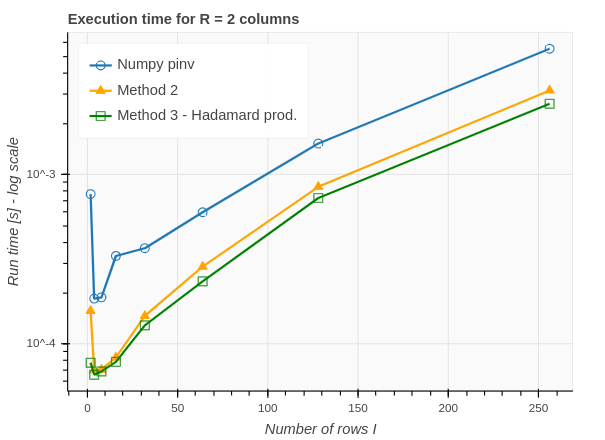
\includegraphics[width=0.55\linewidth]{figs/r2.png}
    \caption{Run time for matrices with $R=2$ columns.}
    \label{r2}
\end{figure}

In Figure \ref{r4}, we can see the computational performance in terms of 
execution time for the case where the matrices have $R = 4$ columns. Again, 
method $2$ and $3$ present the better performances while the method 3 is more 
suitable for small matrices, as can be seen in the figure.

\begin{figure}[H]
    \centering 
    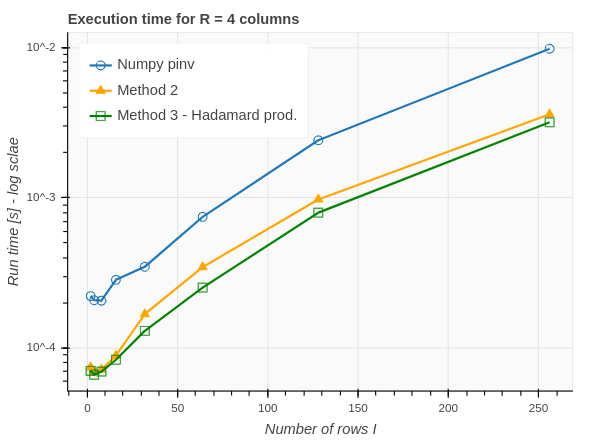
\includegraphics[width=0.55\linewidth]{figs/r4.png}
    \caption{Run time for matrices with $R=4$ columns.}
    \label{r4}
\end{figure}

%------------------------------------------------------------------------------

\noindent
\textbf{Problem 2.} Generate $\bm{X} = \diamond^{N}_{n=1} \bm{A}_{(n)} =
\bm{A}_{(1)} \diamond \dots \diamond \bm{A}_{(N)}$, where every $\bm{A}_{(n)}$ 
has dimensions $4\times 2$, $n = 1, \dots, N$. Evaluate the run time associated 
with the computation of the Khatri-Rao product as a function of the number $N$ 
of matrices for the above method.\\

\noindent \textbf{Solution:}\\

%------------------------------------------------------------------------------
Considering $N \in \{2, 4, 6, 8, 10\}$, we have the result for the rum time 
curve in Figure \ref{p2}. As can be seen in the figure, the \texttt{tensoralg} 
implementation of the nested Khatri-Rao product performs well for a number of 
matrices less than $8$.

\begin{figure}[H]
    \centering 
    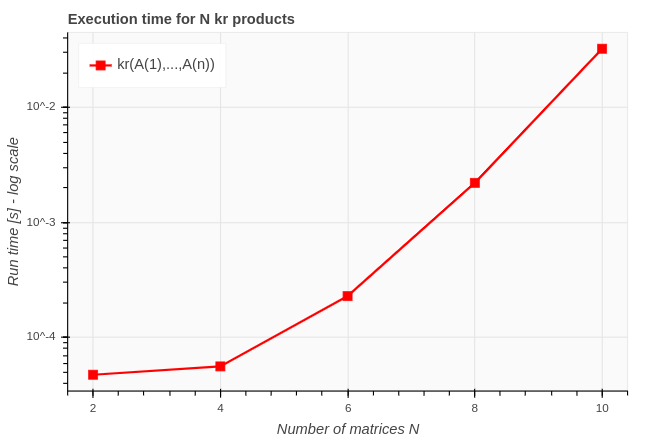
\includegraphics[width=0.55\linewidth]{figs/p2.png}
    \caption{Run time for the N-Khatri-Rao product.}
    \label{p2}
\end{figure}
%------------------------------------------------------------------------------

\end{document}
